\documentclass[a4paper,12pt,twopage,swedish]{article}
\usepackage{amsmath,amssymb,mathrsfs}
\usepackage[utf8]{inputenc}
\usepackage{blindtext}
\usepackage{graphicx}
\usepackage[swedish]{babel}
\usepackage[margin={1in, 1in}]{geometry}
\usepackage{float}
\setlength{\parindent}{0pt}
\renewcommand{\thetable}{\Alph{table}}
%----------------------------------------------------------------------------
\begin{document}

%=================================================================
\title{Stelkroppssimulering}
%----------------------------------------------------------------------------
\author{Tomas Forsyth Rosin, Jonas Zeitler, Emil Axelsson, Karl Johan Krantz}
\begin{titlepage}
\maketitle
\thispagestyle{empty}
\end{titlepage}
%----------------------------------------------------------------------------
\setcounter{page}{1}
\pagenumbering{roman}
\begin{abstract}
\noindent Denna rapport beskriver de fysikaliska koncept och metoder som har använts för att utveckla en fysikmotor för stelkroppar och fjädrar. I rapporten beskrivs metoder för kollisionshantering,  friktionsmodeller och hantering av både kroppar i rörelse och i vila. Även Euler- och Runge-Kutta-metoder för lösning av differentialekvationer behandlas. 
\\
\\Resultatet som presenteras i rapporten är en prototyp av en tvådimensionell fysikmotor implementerad i C++ med grafikramverket OpenGL till stöd.
\end{abstract}
\clearpage
%----------------------------------------------------------------------------
\tableofcontents
\clearpage
%----------------------------------------------------------------------------
\listoffigures
\clearpage
%----------------------------------------------------------------------------
\setcounter{page}{1}
\pagenumbering{arabic}

\section{Inledning}

\subsection{Bakgrund}
Fysiksimulering är en vital del av många moderna datorspel. I spelsammanhang kallas detta för ett spels \emph{fysikmotor}. Att implementera en fysikmotor handlar om att skapa en miljö med regler till vilka en uppsättning objekt måste förhålla sig. I många spel utgörs fysikmotorns bas av en \emph{stelkroppssimulering}, vilket innebär vissa antaganden och förenklingar av verkligheten. Mest påtagligt är att systemets objekt antas vara okomprimerbara, eller stela. Även med dessa förenklingar i beaktning är implementation av en fysikmotor ett komplext problem, som kan lösas på olika sätt beroende på aktuella förutsättningar och tillämpningsområden.

\subsection{Syfte}
Syftet med denna rapport är att beskriva utvecklingen av en fysikmotor, som ska kunna användas i datorspel med tvådimensionell grafik. Motorn ska ha stöd för att simulera kollisioner och friktion mellan stelkroppar modellerade som generella konvexa polygoner. Den ska också innehålla stöd för fjädrar som ska kunna fästas i stelkropparna. Motorn ska producera trovärdiga resultat vid såväl kollisioner som när flera stelkroppar vilar på varandra. Eftersom motorn ska kunna användas till datorspel behöver algoritmerna som används vara tillräckligt tidseffektiva för att tillåta interaktivitet. Motorn ska implementeras i C++ med hjälp av grafikbiblioteket OpenGL varpå resultatet ska utvärderas i rapporten.

%----------------------------------------------------------------------------

\section{Modell}
I modellen som skulle simuleras ingick tre typer av entiteter: rörliga stelkroppar, fasta stelkroppar samt fjädrar. Varje entitet kan ha både konstanta egenskaper och variabla tillstånd, enligt tabell \ref{table:states_and_properties}.

\begin{table}[!h]
	\caption{Tillstånd och egenskaper hos olika entiteter}
	\label{table:states_and_properties}
	\renewcommand{\arraystretch}{1.5}
	\begin{tabular}{|p{2.2cm}|p{2.3cm}|p{2.2cm}|p{2.3cm}|p{2.2cm}|p{2.3cm}|}
		\hline
			\multicolumn{2}{|c|}{\textbf{Rörliga stelkroppar}} & \multicolumn{2}{|c|}{\textbf{Fasta stelkroppar}} & \multicolumn{2}{|c|}{\textbf{Fjädrar}} \\
		\hline
			\textbf{Tillstånd} & \textbf{Egenskaper} & \textbf{Tillstånd} & \textbf{Egenskaper} & \textbf{Tillstånd} & \textbf{Egenskaper} \\
		\hline
			Position & Densitet & & Position & & Infästnings\-punkter \\
			Vinkel & Studs\-koefficient & & Vinkel & & Fjäder\-konstant \\
			Hastighet & & & & & Fri längd \\
			Vinkel\-hastighet & & & & & {} \\
		\hline
	\end{tabular}
\end{table}

Värt att notera i tabellen är att fjädrar inte har några tillståndsvariabler eftersom dessa kan hämtas från de stelkroppar de är fästa i.

%----------------------------------------------------------------------------

\section{Diskret simulering}
Trots att den fysikaliska modell som användes i simuleringen är en förenkling av verkligheten vore det orimligt att försöka beräkna hela förloppet genom att lösa ekvationer analytiskt och göra symboliska integreringar. För simuleringar av detta slag krävs det alltså att modellen diskretiseras i tidsdomänen och att hela simuleringen delas upp i någon form av tidssteg. Många av de matematiska samband som modellen bygger på går att teckna som differentialekvationer (fjäderkrafter, gravitation etc) och det hela resulterar i att en numerisk metod för lösning av differentialekvationer måste väljas och appliceras.

\subsection{Eulers metod}
Ett enkelt sätt att hitta approximativa lösningar till differentialekvationer är att använda Eulers metod, som går ut på att uppdatera alla tillstånd enligt (\ref{eq:euler_method}), där $\bar{y}_t$ är systemets tillstånd vid tidpunkten $t$. I varje tidsteg beräknas ett $\bar{k}$ utifrån rådande samband i det specifika systemet.

\begin{equation}\label{eq:euler_method}
\bar{y}_{t+1} = \bar{y}_t + \bar{k}
\end{equation}

För rörliga stelkroppar betecknar $\bar{y}$ position, hastighet, rotation och rotationshastighet, enligt (\ref{eq:state_vector}), och $\bar{k}$ beräknas som den momentana derivatan av $\bar{y}$ enligt (\ref{eq:state_derivative}).

\begin{equation}\label{eq:state_vector}
\bar{y} = (p_x, p_y, v_x, v_y, \theta, \omega)^T
\end{equation}

\begin{equation}\label{eq:state_derivative}
\bar{k} = \left( \frac{\mathrm{d}p_x}{\mathrm{d}t}, \frac{\mathrm{d}p_y}{\mathrm{d}t}, \frac{\mathrm{d}v_x}{\mathrm{d}t}, \frac{\mathrm{d}v_y}{\mathrm{d}t}, \frac{\mathrm{d}\theta}{\mathrm{d}t}, \frac{\mathrm{d}\omega}{\mathrm{d}t} \right) ^T = (v_x, v_y, a_x, a_y, \omega, \alpha)^T
\end{equation}

\subsection{Runge-Kutta-metoder}
Ett problem med Eulers metod är att den leder till instabilitet då den används för att simulera komplexa system. För att klara av att simulera system av fjädrar i fysikmotorn användes en Runge-Kuttalösning av ordning 4. Det innebär att fyra tillståndsderivator ($k_1$-$k_4$), utgående från initialtillståndet $y_t$, beräknas och kombineras till en lösning.

\begin{equation}\label{eq:runge-kutta_sum}
\bar{y}_{t+1} = \bar{y}_t + frac{1}{6}(\bar{k}_1 + 2\bar{k}_2 + 2\bar{k}_3 + \bar{k}_4)
\end{equation}

\begin{equation}\label{eq:runge-kutta_k1}
\bar{k}_1 = f(\bar{y}_t)
\end{equation}

\begin{equation}\label{eq:runge-kutta_k2}
\bar{k}_2 = f(\bar{y}_t + \frac{1}{2}\bar{k}_1)
\end{equation}

\begin{equation}\label{eq:runge-kutta_k3}
\bar{k}_3 = f(\bar{y}_t + \frac{1}{2}\bar{k}_2)
\end{equation}

\begin{equation}\label{eq:runge-kutta_k4}
\bar{k}_4 = f(\bar{y}_t + \frac{1}{2}\bar{k}_3)
\end{equation}

I (\ref{eq:runge-kutta_k1}-\ref{eq:runge-kutta_k4}) beräknar $f$ den momentana derivatan givet ett tillstånd och i (\ref{eq:runge-kutta_sum}) vägs dessa derivator samman till ett resultat som, med en mindre avvikelse än Euler-metoden, approximerar medelderivatan mellan två tidssteg.

\subsection{En hybrid}
Medan den ovan beskrivna Runge-Kutta metoden lämpar sig för att lösa differentialekvationer är den svår att tillämpa på kollisioner mellan kroppar, då hastigheter och vinkelhastigheter ska ändras momentant. Metoden som implementerades var därför en hybrid mellan de två ovannämda tillvägagångssätten, där Runge-Kutta av ordning fyra användes för att simulera fjäderkrafter, gravitation och obehindrade förflyttningar, medan en Euler-metod applicerades i slutet av varje steg för att lösa och ge respons på de kollisioner som uppträtt under tidssteget.




%----------------------------------------------------------------------------




\section{Kollisionsdetektion}

\subsection{Detektionsmetod}
Ett första steg mot att simulera stelkroppars interaktion är att detektera alla kolliderande polygoner i scenen. Att två kroppar i ett diskret system ligger \emph{dikt an} varandra är sällsynt. Vanligare är att de \emph{interpenetrerar} varandra, d.v.s. att ett hörn hos en kropp ligger inuti en annan kropp.

\subsubsection{Separating Axis Test}
För att utreda eventuell interpenetration mellan två givna objekt kan SAT\cite[s.~29]{vella08} \emph{(Separating Axis Test)} användas. Testet kan avgöra om kropparna \emph{inte} kolliderar genom att hitta en vektor på vilken objektens punkter projiceras på disjunkta intervall (Figur \ref{fig:hejhej}). Ett högre antal vektorer ökar beräkningstiden men också sannolikheten för ett korrekt resultat.

\subsubsection{Gilbert-Johnson-Keerthi}
\label{sec:gjk}
För att inte göra avkall på noggrannheten implementerades istället en annan metod, GJK \cite[s.~30]{vella08} \emph{(Gilbert-Johnson-Keerthi)}. Eftersom metoden kan utesluta fler möjliga kollisioner kommer senare beräkningar kräva mindre tid. GJK bygger på Minkovskidifferensen mellan de två kropparna, definierad enligt (\ref{eq:minkowski_difference}).

\begin{equation}\label{eq:minkowski_difference}
\chi_1 \ominus \chi_2 = \{ x_1 - x_2|x_1 \in \chi_1, x_2 \in \chi_2 \}
\end{equation}

De två kropparna korsar varandra om, och endast om, polygonen som Minkovskidifferensen renderar innehåller origo (Figur \ref{fig:gjk}). GJK-algoritmen utreder detta utan att behöva ta alla punkter i beaktning vilket resulterar i lägre komplexitet i beräkningarna \cite{bergen99}.

\begin{figure}[H]
\centering
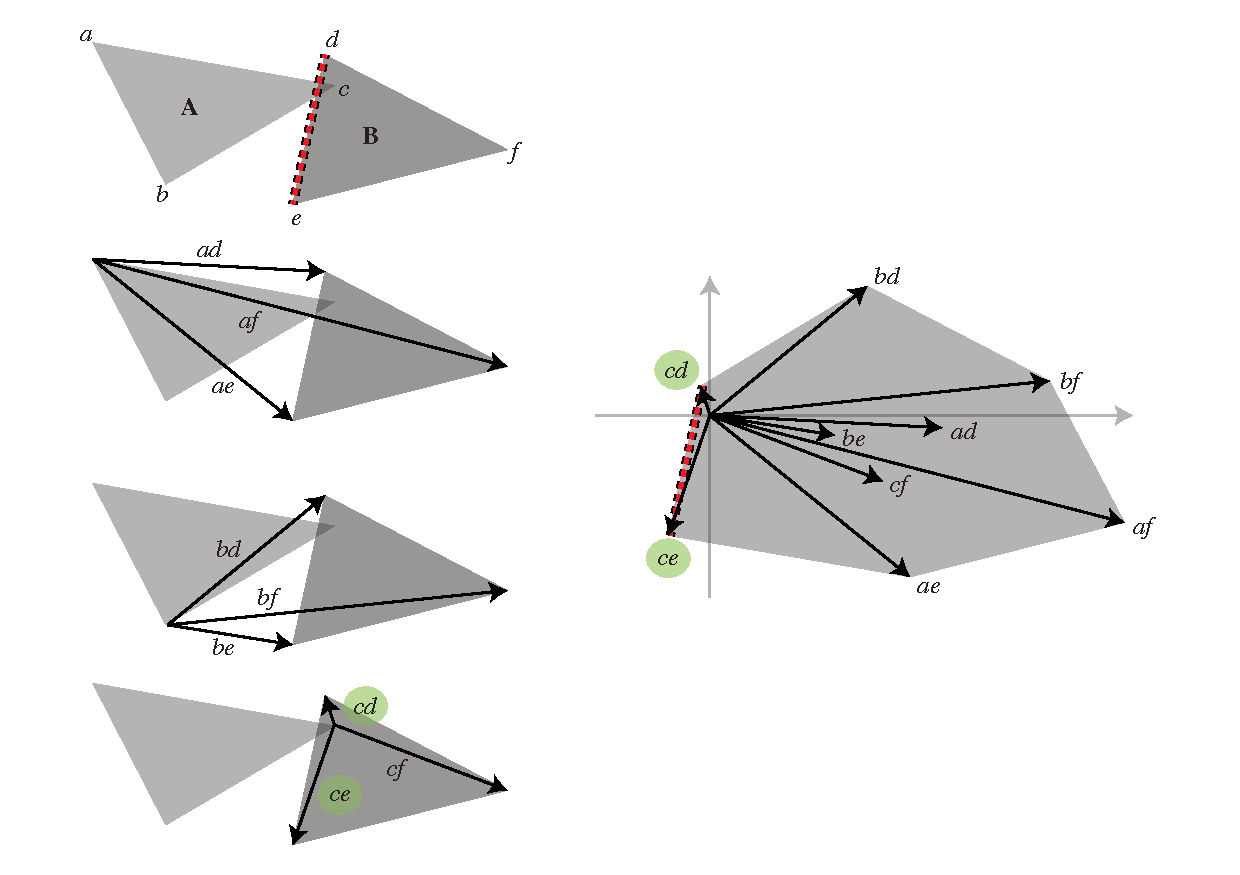
\includegraphics[width=1\textwidth]{illustrations/gjk.pdf}
\caption{Minkowskidifferensen och dess uppbyggnad}
\label{fig:gjk}
\end{figure}

\subsection{Optimering}

Att i varje tidssteg använda GJK-algoritmen för att testa kollision mellan alla kroppar i en scen skulle innebära omfattande beräkningar, vilket skulle tvinga ner fysikmotorns prestanda betydligt. För att undvika dessa beräkningsmängder görs först olika bedömningar av vilka kroppar som riskerar att kollidera varefter de mer komplexa kollisionsdetektorerna appliceras endast på dessa par.

\subsubsection{Bounding boxes}
Det är mer beräkningseffektivt att kontrollera om två kvadrater överlappar varandra än att använda GJK-algoritmen. Därför implementerades en algoritm som räknar ut de minsta kvadrater som garanterat omger alla hörnpunkter hos stelkropparnas polygoner. Detta koncept kallas \emph{bounding boxes}. Naturligtvis går det inte att säkerställa kollsisioner med denna metod utan bara avfärda dem (Figur \ref{fig:bounding_boxes}).

\begin{figure}[H]
\centering
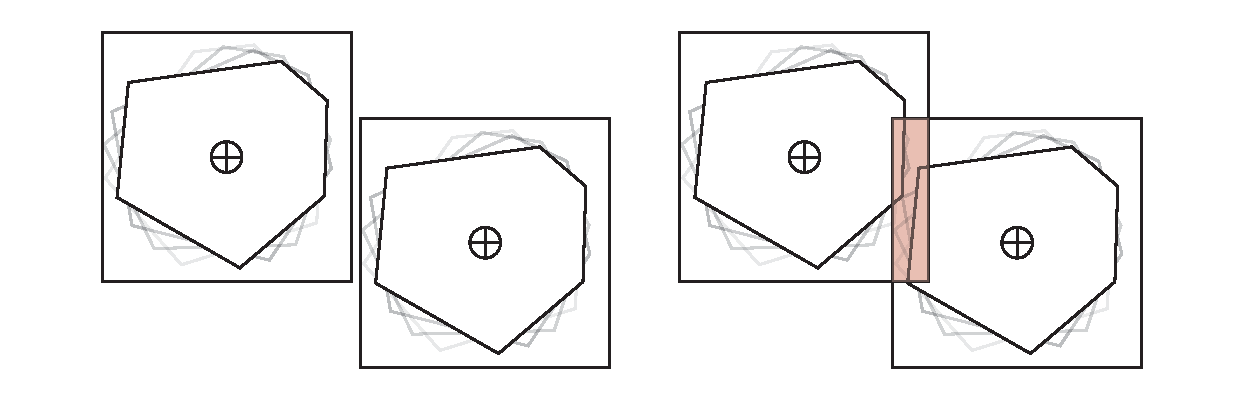
\includegraphics[width=1\textwidth]{illustrations/boundingbox.pdf}
\caption{Bounding boxes och hur de skär varandra}
\label{fig:bounding_boxes}
\end{figure}

\subsubsection{Quadträd}

En ytterligare optimering som kan göras är att använda ett quadträd för att dela upp simuleringsomådet och på detta sätt avgöra vilka kroppar som potentiellt kan ge upphov till kollisioner. Ett quadträd är en datastruktur som delar in en stor område i fyra mindre likformiga områden, varpå dessa rekursivt klyvs på samma sätt tills önskad granularitet uppnås. Genom att tidigt avfärda kollisioner mellan objekt som ligger i skiljda noder i quadträdet behöver betydligt färre  par av kroppar skickas till Bounding box-testet. 
\\
\\Ett quadträd implementerades genom att skapa kvadratiska noder som var och en gavs ett register av vilka stelkroppar som befinner sig inuti dem. Allteftersom kroppar lämnar och äntrar noder uppdateras varje nods register. Snabba uppslagningar kan därmed göras i kollisionsdetektionsprocessen. I figur  \ref{fig:quadtree} visas hur noder som innehåller mindre än två stelkroppar helt kan uteslutas från vidare kollisionsdetektion.

\begin{figure}[H]
\centering
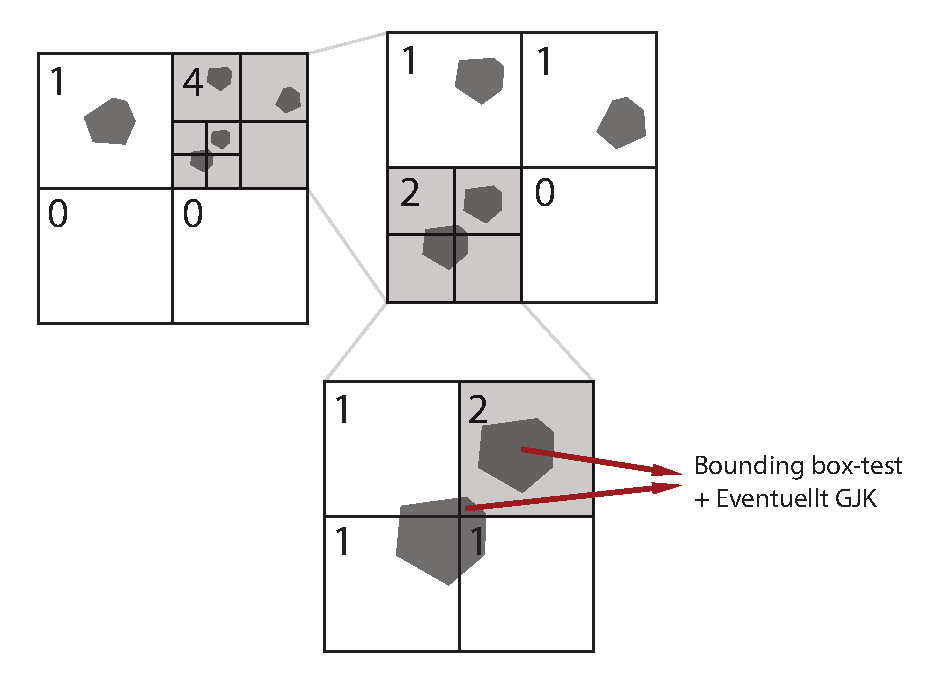
\includegraphics[width=0.8\textwidth]{illustrations/quadtree.pdf}
\caption{Quadträdets iterativa uppdelning}
\label{fig:quadtree}
\end{figure}


%----------------------------------------------------------------------------


\section{Kollisionslösning}
Att två objekt interpenetrerar varandra representerar inget verkligt fysikaliskt förlopp. Det första som därför måste göras när en sådan händelse upptäckts är att flytta ut objekten från varandra. En metod för detta är att hitta det tidssteg mellan innevarande och föregående bildruta då objekten kolliderade. En analytisk lösning är emellertid komplicerad att implementera med tanke på translations- och rotationshastigheter. En enklare metod är att hitta den punkt hos polygon A som interpenetrerar längst och betrakta den sida på polygon B som ligger närmast denna punkt som en trolig kollisionssida. Hur objekten sedan separeras från varandra går att lösa på olika sätt - linjärt eller icke-linjärt.

\subsection{Expanding Polytope Algorithm (EPA)}
I denna tillämpning användes metoden EPA (Expanding Polytope Algorithm) för att hitta penetrationspunkten och en vektor mellan denna punkt och kollisionssidan, nedan kallad penetrationsvektorn. I det konvexa höljet av Minkowskidifferensen, beskriven i avsnitt \ref{sec:gjk}, kommer den linje med minst avstånd till origo att vara av intresse. De punkter som spänner upp denna linje har genererats utifrån penetrationspunkten, i  BEHÖVER FIGUR benämnd c, och de två punkter, d och e, som spänner upp kollisionssidan.


\subsection{Linjär Kollisionslösning}

\begin{figure}[H]
	\centering
	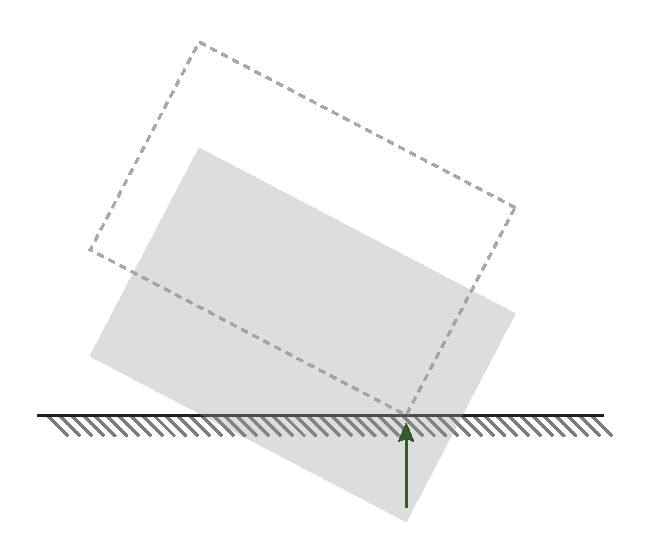
\includegraphics{illustrations/linear.pdf}
	\caption{Exempel på linjär utflyttning}
	\label{fig:linear}
\end{figure}

En linjär kollisionslösning är det enklaste sättet att lösa interpenetration. Penetrationen löses sådant att kropparna a och b (Figur \ref{fig:linear}) translateras i penetrationsvektorns positiva respektive negativa riktning. Hur stor del av penetrationsvektorn respektive kropp skall translateras beräknas med avseende på dess omvända relativa massa enligt (\ref{eq:impulse_part}).

\begin{equation}\label{eq:impulse_part}
	J_{part} = \frac{m_i}{m_1+m_2}
\end{equation}

Att translatera en rörlig kropp ut från en stationär kropp utan att påverka dess hastighet medför en förändring av systemets energi. För att motverka detta beräknas hastigheten om med avseende på utflyttningen och gravitationen.

\begin{equation}\label{eq:v_magnitude}
	|\bar{v}| = \sqrt{|v^{2}-2\cdot|g_y| \cdot t_y|}
\end{equation}

Ekvation (\ref{eq:v_magnitude}) beskriver den nya hastigheten $v$ där $t$ är kroppens utflyttningsvektor och $g$ är den aktuella gravitationen för systemet.

\subsection{Icke-linjär kollisionslösning}
Linjära lösningar för interpenetration skapar problem för kroppar i vila. Detta eftersom gravitationen påverkar kropparna vilket resulterar i interpenetration med underlaget. Detta resulterar i sin tur i en linjär utflytt med avseende på den punkt med längst penetrationsvektor. För kroppar i vila innebär detta att de kommer vibrera istället för att ligga stilla. Dessutom kan det visas att oönskad friktion introduceras i systemet. Ett förslag till förbättring är att dela upp utflyttning av en kropp till två komponenter. En linjär förflyttningskomponent med avseende på kroppens tröghet (\ref{eq:mass_mass_inertia_part}) och en rotationskomponent med avseende på kroppens tröghetsmoment (\ref{eq:inertia_mass_inertia_part}).

\begin{equation}\label{eq:mass_mass_inertia_part}
	lm_i = \frac{\frac{1}{m_i}}{\frac{1}{m_1} + \frac{1}{m_2} + \frac{1}{I_1} + \frac{1}{I_2}}
\end{equation}

\begin{equation}\label{eq:inertia_mass_inertia_part}
 	am_i = \frac{\frac{1}{m_i}}{\frac{1}{m_1} + \frac{1}{m_2} + \frac{1}{I_1} + \frac{1}{I_2}}
\end{equation}

I simuleringen implementerades endast den linjära utflyttningskomponenten (\ref{eq:mass_mass_inertia_part}) och sedan en explicit lösning (Figur \ref{fig:nonlinear}) för hur kroppen ska roteras ut.

\begin{figure}[H]
	\centering
	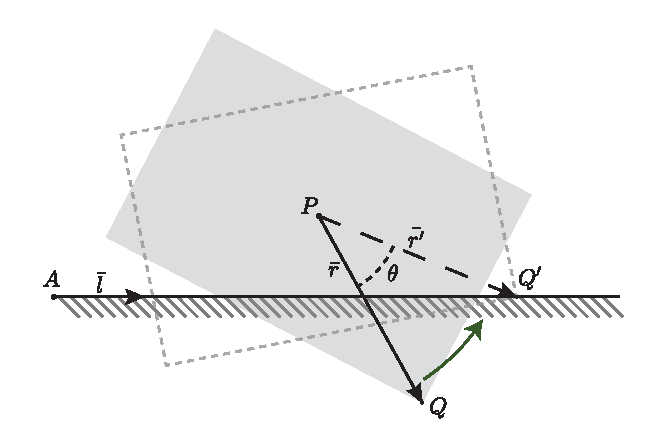
\includegraphics{illustrations/nonlinear.pdf}
	\caption{Exempel på icke-linjär utflyttning}
	\label{fig:nonlinear}
\end{figure}

Metoden innebär att lösa ett ekvationssystem med fyra rötter och sedan testa vilken lösning som ger den optimala, dvs. minsta,  rotationen ut.
\begin{equation} \label{eq:nonlinear_1}
	Q' = P + \bar{r}' = A + s \cdot \bar{l}
\end{equation}

\begin{equation}\label{eq:nonlinear_2}
	|\bar{r}|^2 = |\bar{r}'|^2 = (Q-P)^2 = (Q' - P)^2
\end{equation}

\begin{equation}\label{eq:nonlinear_3}
	\theta = \arccos{\frac{\bar{r}\cdot\bar{r} '}{|\bar{r}|^2}}
\end{equation}

Från (\ref{eq:nonlinear_1}) och (\ref{eq:nonlinear_2}) löses $\bar{r}'$ut och rotationen beräknas enligt (\ref{eq:nonlinear_3}).

För kroppar med stor massa blir den linjära komponenten liten. Djupa penetrationer kan då resultera i att rotationen förvärrar interpenetrationen. I dessa fall kan en nedre gräns för den linjära komponenten införas för att balansera förhållandet mellan rotation och translation \cite{millington07}.



%----------------------------------------------------------------------------



\section{Kollisionsrespons}
\subsection{Impulsbaserade system}
I det system som simuleras måste någon representation av krafter mellan kroppar finnas. En vanlig förenkling är att se krafter som momentana händelser i tiden. Detta introducerar begreppen impuls och rörelsemängd. Impulser kan relateras till krafter enligt (\ref{eq:force_to_impulse}).

\begin{equation}\label{eq:force_to_impulse}
\bar{J} = \int_{\Delta t}^{} \bar{F} \ dt = \int_{\Delta t}^{} m\bar{a} \ dt = m\bar{v}
\end{equation}

Den aktuella implementationen av (\ref{eq:force_to_impulse}) innehöll inget begrepp om tid utan $t$ representerades istället av ett simuleringssteg.

\subsubsection{Praktiskt förlopp}
Då en kollision detekteras ska fysikmotorn lösa vilka krafter som uppstår mellan kropparna. En nödvändig förenkling är att endast hantera kollisioner som sker mellan hörn och sida för kroppar. Dessa är de absolut vanligast förekommande kollisionerna och det är ur optimeringssynpunkt inte värt att ta hänsyn till andra typer av kollisioner. Den data som finns tillgänglig för kollisionsrespondern är:

\begin{itemize}
\item \text{De kroppar som ingår i kollisionen}
\item \text{I vilken punkt kollisionen sker}
\item \text{Normalvektorn för kollisionsplanet/-sidan}
\end{itemize}

\begin{figure}[H]
	\centering
	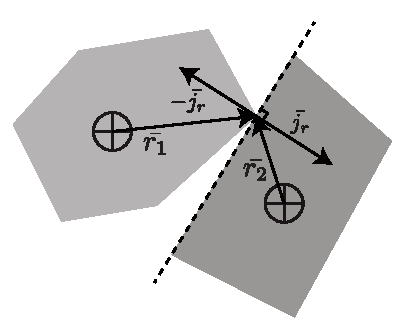
\includegraphics{illustrations/impulse.pdf}
	\caption{Impulser i kollisionspunkten}
	\label{fig:impulse}
\end{figure}

Lösningen för den resulterande impulsens magnitud, $j_r$ , illustreras bäst genom att först förstå hur impulsen appliceras på kropparnas hastigehet och vinkelhastighet.

\begin{equation}\label{eq:impulse_apply_linear}
\bar{v}_1' = \bar{v}_1 + \frac{j_r}{m_1}\hat{n}, \ \bar{v}_2' = \bar{v}_2 + \frac{j_r}{m_2}\hat{n}
\end{equation}

\begin{equation}\label{eq:impulse_apply_angular}
\omega_1' = \omega_1 + \frac{j_r}{I_1}(\bar{r}_1 \times \hat{n}), \ \omega_2' = \omega_2 + \frac{j_r}{I_2}(\bar{r}_2 \times \hat{n})
\end{equation}

För (\ref{eq:impulse_apply_linear}-\ref{eq:impulse_apply_angular}) är alla parametrar kända, utom $\bar{v}_i'$, $\omega_i'$ och $j_r$ . Vektorn $\bar{r}_i$ är vektorn från $i$:te kroppens masscentrum till kollisionspunkten, $P$, vilken är gemensam för båda kropparna i kollisionen. Normalvektorn, $\hat{n}$, ges som inparameter från EPA. Punktens hastighet för respektive kropp beräknas enligt (\ref{eq:collision_point_velocity}).

\begin{equation}\label{eq:collision_point_velocity}
\bar{v}_{i_P} = \bar{v}_i + \omega \times \bar{r}_i
\end{equation}

\begin{equation}\label{eq:collision_restitution}
\bar{v}_r' \cdot \hat{n} = -e\bar{v}_r \cdot \hat{n}
\end{equation}
\begin{equation}\label{eq:separating_velocity}
\bar{v}_r = \bar{v}_{1_P} - \bar{v}_{2_P}, \ \bar{v}_r' = \bar{v}_{1_P}' - \bar{v}_{2_P}'
\end{equation}

Ekvation (\ref{eq:collision_restitution}) relaterar kropparnas separationshastighet (\ref{eq:separating_velocity}), före och efter kollisionen. Parametern $e$ anger materialens studskoefficient. Genom substitution av (\ref{eq:impulse_apply_linear}-\ref{eq:collision_point_velocity}) i (\ref{eq:collision_restitution}) kan kollisionsimpulsen lösas ut enligt (\ref{eq:impulse_magnitude}).

\begin{equation}\label{eq:impulse_magnitude}
j_r = \frac{-(1+e)\bar{v}_r \cdot \hat{n}}
{\frac{1}{m_1}+\frac{1}{m_2}+(\frac{1}{I_1}(\bar{r}_1 \times \hat{n}) \times \bar{r}_1+\frac{1}{I_2}(\bar{r}_2 \times \hat{n}) \times \bar{r}_2)\cdot \hat{n}}
\end{equation}

Genom detta skapas en grundläggande teori om hur kollisioner ska bete sig i simuleringen. En impuls beräknas i (\ref{eq:impulse_magnitude}) och appliceras sedan i (\ref{eq:impulse_apply_linear}) och (\ref{eq:impulse_apply_angular}).
\\
\\Under implementationen introducerades ett specialfall för kollision mellan rörlig och icke-rörlig kropp. Detta resulterade i en förenklad impulsmodell enligt (\ref{eq:impulse_magnitude_simple}).

\begin{equation}\label{eq:impulse_magnitude_simple}
j_r = \frac{-(1+e)\bar{v}_r \cdot \hat{n}}
{\frac{1}{m_1}+\frac{1}{I_1}(\bar{r}_1 \times \hat{n}) \times \bar{r}_1 \cdot \hat{n}}
\end{equation}

Ekvation (\ref{eq:impulse_magnitude_simple}) kan likställas med att sätta den stationära kroppens massa och tröghetsmoment till $\infty$.

\subsection{Penalty-baserade system}
Vid kollision mellan två kroppar i verkligheten är det två kontinuerliga motriktade krafter som verkar på objekten, dessa krafter är aktiva över en kort tidsperiod, något som gör att det är mer korrekt att använda än impulsbaserad kollisionslösning.
Vid vilande kontakt är detta dock inte en lösning som ger trovärdiga resultat, vilket diskuterats ovan. Detta eftersom det sällan endast är ett hörn som är i kontakt mellan två kroppar i vila. Vid implementation ansågs därför att en penalty-baserad kollisionslösning var mer lämplig i dessa fall.

Metoden medför att en utflyttning ej sker, objekt använder sig istället av mindre impulser för för att fjädra ifrån varandra. Detta kan illustreras (Figur ~\ref{fig:penalty}) som dämpade fjädrar som spänns mellan kropparna längs penetrationsvektorn.

\begin{figure}[H]
	\centering
	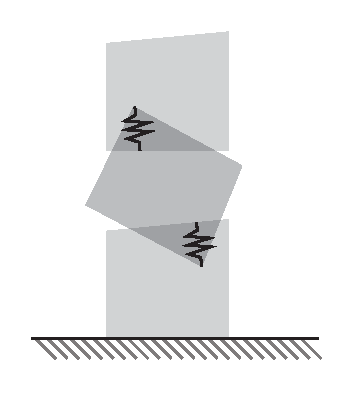
\includegraphics{illustrations/penalty.pdf}
	\caption{Tillämpning av dämpade fjädrar som kontaktmodell}
	\label{fig:penalty}
\end{figure}

Ekvation (\ref{eq:penalty_impulse}) anger den impuls $J$ som ger fjädringen på båda objekten.

\begin{equation}\label{eq:penalty_impulse}
\bar{J} = C \cdot \bar{P}
\end{equation}

Där $C$ är en framerate-baserad konstant och $\bar{P}$ är penetrationsvektorn mellan de två objekten.

\subsubsection{Övergång}
En övergång mellan de två lösningsmetoderna är aktuell först när objekt vilar på varandra, vilket innebär att deras relativa hastighet i kollisionspunkten är låg.
En tröskel som varierar med de aktuella egenskaperna hos systemet kan ge mer korrekta lösningar. Vid empiriska tester så sattes emellertid en fast tröskel för övergången mellan metoderna.



%----------------------------------------------------------------------------



\section{Krafter i impulsbaserade system}

\subsection{Kraftgeneratorer}

Hittills har endast momentana krafter mellan objekt diskuterats. Det har också poängterats att detta är en förenkling av vad som sker i stötar och kontakt. En kollision mellan två objekt orsakar kompression hos materialen i respektive objekt vilket i sin tur ger upphov till krafter mellan kropparna \cite{newton87}.
\\
\\Vissa fysikmotorer delar upp varje tidssteg i mindre delar och kan på så sätt erhålla en bättre approximation för vissa krafter. Dessa metoder kallas tidsderiverande. En tidsderiverande fysikmotor kan använda simuleringsmetoder, t.ex. Runge-Kutta, som kräver information om  flera olika tillstånd hos systemet.
\\
\\I simuleringen implementeras kraftgeneratorer för gravitation och fjäderkrafter.

%\begin{equation}\label{eq:impulse_force_relation}
%J = \int\limits_{\Delta t} F \,dt\
%\end{equation}

\subsection{Fjäderkrafter}
En fysikmotor som implementerar massa-fjäder-system och harmonisk rörelse kräver att det finns mer sofistikerade simuleringsmetoder än Euler för icke-triviala fall. Detta motiverar att låta fjäderkrafter vara kraftgeneratorer och därmed simuleras med en Runge-Kuttalösning.
\\
\\Hookes lag beskriver den kraft en fjäder påverkar andra objekt med. Kraften beror av hur utdragen eller sammanpressad fjädern är. Det vill säga, kraftgeneratorn behöver endast positionen av fjäderns infästningspunkter för att beräkna fjäderkraften. 

\begin{equation}\label{eq:hookes_law}
f = - k \cdot \Delta l
\end{equation}

I (\ref{eq:hookes_law}) är $k$  fjäderkonstant och $\Delta l$ anger hur utdragen eller sammanpressad fjädern är. Lösningen för (\ref{eq:hookes_law}) ger endast  kraftens magnitud, för en flerdimensionell simulering utökas ekvationen till att även innehålla kraftens riktning (\ref{eq:hookes_law_2dim}).

\begin{equation}\label{eq:hookes_law_2dim}
f = - k (|\bar{d}| - l_0)\hat{d}
\end{equation}

\begin{equation}\label{eq:hookes_extremities}
\bar{d} = x_A - x_B
\end{equation}
Parametrar $x_A$ och $x_B$ (\ref{eq:hookes_extremities}) är infästningspunkter med avseende på position och rotation för ett tillstånd $y_t$.
\\
\\Ett viktigt resultat för Hookes lag är att den resulterande kraften $f$ verkar lika mycket i fjäderns båda ändar.

\subsection{Friktion}

Den allra vanligaste friktionsmodellen är Coloumbs modell. Den baserar sig i att den friktionskraft som påverkar en kropp är proportionell mot normalkraften mellan kroppen och underlaget. Modellen är egentligen en sammanslagning av två modeller, statisk och dynamisk friktion.

\begin{equation}\label{eq:static_friction}
\bar{f_s} = \mu_s \cdot \bar{N}
\end{equation}

\begin{equation}\label{eq:dynamic_friction}
\bar{f_s} = \mu_d \cdot \bar{N}
\end{equation}

Där den statiska modellen (\ref{eq:static_friction}) används för kroppar i vila och den dynamiska (\ref{eq:dynamic_friction}) för kroppar i rörelse. Båda modellerna kan endast ge upphov till friktionskrafter som är proportionella mot de yttre krafter som verkar på kroppen. Friktionskrafter verkar i kontaktplanets tangentriktning, $\bar{t}$.

\begin{equation}\label{eq:friction_force_final}
f_t =\begin{cases}
    -(\bar{f}_{ext} \cdot \hat{t})\hat{t}, & \bar{v}_r = \bar{0}, \bar{f}_{ext} \cdot \hat{t} \le \bar{f}_s \\
    -\bar{f}_s \cdot \hat{t}, & \bar{v}_r = \bar{0}, \bar{f}_{ext} \cdot \hat{t} > \bar{f}_s \\
    - \bar{f}_d \cdot \hat{t} , & \bar{v}_r \ne \bar{0}
  \end{cases}
\end{equation}

Enligt (\ref{eq:friction_force_final}) kan endast en extern kraft i kontaktplanet som överstiger den maximala statiska friktionskraften sätta en kropp i rörelse. I annat fall motverkas kraften av en lika stor friktionskraft vilket medför att kroppen förblir vilande.
\\
\\Den friktionsmodell som används i simuleringen är ingen kraftgenerator utan tar endast hänsyn till impulser vid kontakt. En omskrivning av (\ref{eq:static_friction}-\ref{eq:friction_force_final}) ger den friktionsimpuls som motsvarar $\bar{f}_t$.

\begin{equation}\label{eq:static_friction_impulse}
\bar{j}_s = \mu_s \cdot \bar{j}_r
\end{equation}

\begin{equation}\label{eq:dynamic_friction_impulse}
\bar{j}_d = \mu_d \cdot \bar{j}_r
\end{equation}

\begin{equation}\label{eq:friction_impulse_final}
j_f =\begin{cases}
    -(m\bar{v}_r \cdot \hat{t})\hat{t}, & \bar{v}_r = \bar{0}, m\bar{v}_r \cdot \hat{t} \le \bar{j}_s \\
    -\bar{j}_s \cdot \hat{t}, & \bar{v}_r = \bar{0}, m\bar{v}_r \cdot \hat{t} \ge \bar{j}_s \\
    - \bar{j}_d \cdot \hat{t} , & \bar{v}_r \ne \bar{0}
  \end{cases}
\end{equation}

Friktionsimpulsen (\ref{eq:friction_impulse_final}) appliceras samtidigt som kollisionsimpulsen för respektive kropp och kollision. Ekvation (\ref{eq:static_friction_impulse}-\ref{eq:friction_impulse_final}) är en ideal [Gravitas] friktionslösning för impulsbaserade system. Det kan emellertid visas att (\ref{eq:static_friction_impulse}) och (\ref{eq:dynamic_friction_impulse}) inte ger energibevarande lösningar för höga värden på $\mu_s$ och $\mu_d$.
\\
\\Friktion simulerades utan hänsyn till friktionstal mellan specifika material. Istället har en naiv förenkling till de allra mest grundläggande egenskaperna implementerats enligt (\ref{eq:friction_simple}).

\begin{equation}\label{eq:friction_simple}
\bar{j}_r = \frac{|\bar{v}_r \cdot \hat{n}_{\perp}|}{\frac{1}{m_1}+\frac{1}{m_2}+\frac{1}{I_1}(\bar{r}_{1_{\perp}} \cdot \hat{n}_{\perp})^2+\frac{1}{I_2}(\bar{r}_{2_{\perp}} \cdot \hat{n}_{\perp})^2}
\end{equation}

Ekvation (\ref{eq:friction_simple}) kan jämföras med (\ref{eq:impulse_magnitude}) som bygger på samma princip.

%----------------------------------------------------------------------------



\section{Resultat}
Under projektet har en prototyp till en fysikmotor utvecklats. Motorn kan lösa ett antal sofistikerade uppsättningar av konvexa stelkroppar och producera trovärdiga resultat. 
Exempel på detta är:

\begin{itemize}
\item \text{Energibevarande kollisioner med translation och rotation (Figur ~\ref{fig:general})}
\item \text{Vilande kroppar (Figur ~\ref{fig:resting})}
\item \text{Komplexa massa-fjäder-system (Figur ~\ref{fig:vagn_that_can_go})}
\item \text{Kollisionsdetektion för godtyckliga konvexa objekt}
\end{itemize}

\begin{figure}[H]
	\centering
	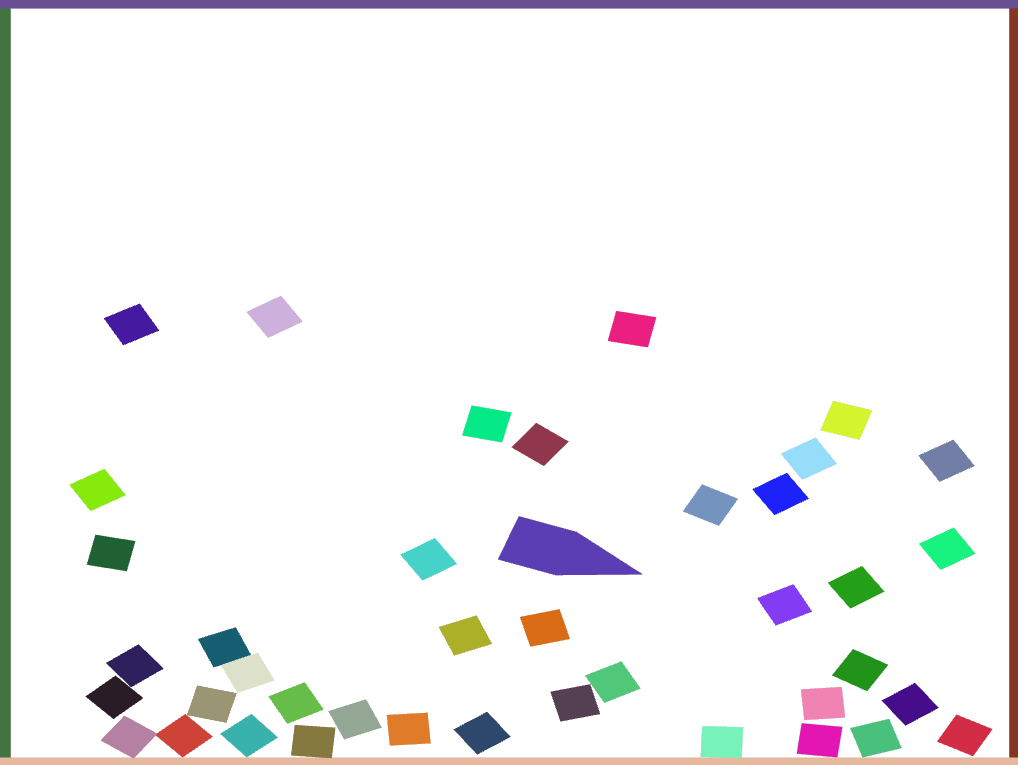
\includegraphics[width=0.9\textwidth]{illustrations/printscreen_general.png}
	\caption{Energibevarande kollisioner}
	\label{fig:general}
\end{figure}
\begin{figure}[H]
	\centering
	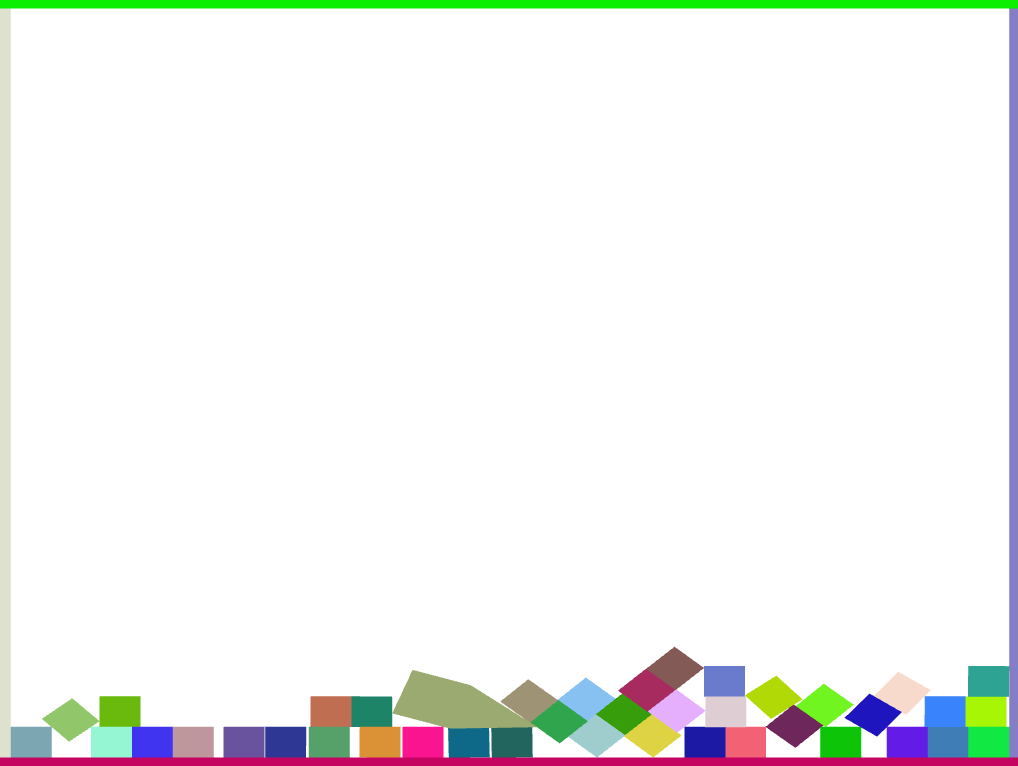
\includegraphics[width=0.9\textwidth]{illustrations/printscreen_resting.png}
	\caption{Vilande kroppar}
	\label{fig:resting}
\end{figure}
\begin{figure}[H]
	\centering
	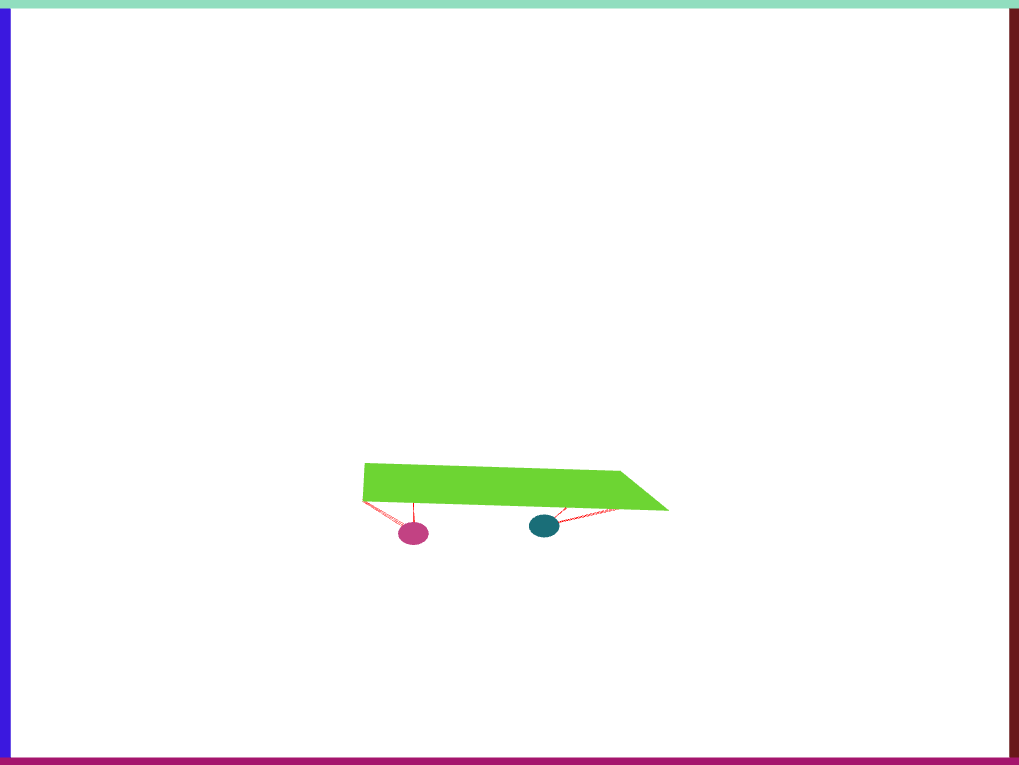
\includegraphics[width=0.9\textwidth]{illustrations/printscreen_a_vagn_that_can_go.png}
	\caption{Massa-fjäder-system}
	\label{fig:vagn_that_can_go}
\end{figure}



%----------------------------------------------------------------------------



\section{Diskussion}


\subsection{Kontaktgrupper}
En möjlig optimering som har diskuterats under projektets gång har varit att gruppera ihop statiska kontakter mellan kroppar. Denna optimering skulle möjliggöra att gruppera ihop kroppar som under en längre tid kolliderat och lägga dessa i vila. Inga beräkningar skulle då behöva utföras på dessa objekt då deras tillståndsvariabler ej förändras när de ligger i detta tillstånd. Den implementation som har beskrivits i rapporten har den svagheten att GJK-algoritmen kommer att behöva köras mellan alla objekt som vilar mot varandra i varje tidssteg.

\subsection{Konkava Kroppar}
Att fysikmotorer begränsas till att hantera konvexa polygoner är en vanlig förenkling då det resulterar i en adekvat kompromiss mellan prestanda och generalitet. Konkava former skulle framförallt kräva en mer komplex metod för att detektera kollisioner.

Möjliga lösningar på detta problem är att antingen använda konkava kroppars konvexa hölje vid kollisionsdetektion, eller att segmentera den konkava kroppen till flera mindre konvexa kroppar.

\subsubsection{Konvext Hölje}
Ett konkavt objekt kan utvidgas till att vara ett konvext objekt. Det kallas att hitta det konvexa höljet till kroppen. Syftet med detta är att förenkla kroppens kollisionsberäkningar \cite[s.~29]{avis97}.

\subsubsection{Segmentering}
Några algoritmer där fysikmotorn automatiskt delar upp konvexa kroppar till konkava har studerats.
Implementationen är dock komplex nog att utvecklingsteamet bortsåg från att implementera detta och istället fokusera på mer komplexa fysikaliska samband.



\subsection{Simuleringsmetoder}
I många fall i rapporten har påpekats att det gjorts förenklingar av förlopp som skulle vinna på att simuleras med mer komplexa metoder. Exempel på detta är friktion och penalty-metoder.  Runge-Kuttametoden infördes sent i utvecklingsarbetet. Detta är en bidragande faktor till att en stor del av implementationen fortfarande använder Eulermetod. Att föra över ovan nämnda områden från simulering med en sekventiell metod till en simultan Runge-Kuttametod har hög prioritet för eventuellt fortsatt arbete.


\clearpage
%=================================================================
\begin{thebibliography}{9}

\bibitem{vella08}
  Vella Colin,
  \emph{Gravitas: An extensible physics engine framework using object-oriented and design pattern-driven software architecture principles}.
  2008.

\bibitem{millington07}
  Millington Ian,
  \emph{Game Physics Engine Development}.
  2007.

\bibitem{kumar12}
  Kumar Ashok, Etheredge Jim, Boudreaux Aaron,
  \emph{Algorithmic and Architectural Gaming Design: Implementation and Development}.
  2012.

\bibitem{bergen99}
  Van den Bergen Gino,
  \emph{A Fast and Robust GJK Implementation for Collision Detection of Convex Objects, Journal of Graphics Tool}.
  4:2, 7-25,
  1999.

\bibitem{newton87}
  Newton Isaac
  \emph{Philosophiæ Naturalis Principia Mathematica}.
  1687.

\bibitem{avis97}
  Avis David, Bremnes David, Seidel Raimund,
  \emph{How good are convex hull algorithms?}.
  1997.

\end{thebibliography}
\end{document} 